% Preamble
\documentclass[12pt]{article}

% Packages
\usepackage[a4paper, includefoot,
  left=3cm, right=1.5cm,
  top=2cm, bottom=2cm,
headsep=1cm, footskip=1cm]{geometry}
\usepackage{amsmath}
\usepackage{amssymb}
\usepackage[T2A]{fontenc}
\usepackage[utf8]{inputenc}
\usepackage[english, russian]{babel}
\usepackage{stmaryrd}
\usepackage{pdfpages}
\usepackage{graphicx}
\usepackage{wrapfig}
\usepackage{amsthm}
\usepackage{framed}
\usepackage{xcolor}
\usepackage{color}
\usepackage[unicode]{hyperref}

\hypersetup{
  colorlinks=true,
  linkcolor=black,
  urlcolor=blue,
}

%new calligraphic font for subspaces 
\usepackage{euscript}
\newcommand{\cA}{\EuScript{A}}
\newcommand{\cB}{\EuScript{B}}
\newcommand{\cC}{\EuScript{C}}
\newcommand{\cD}{\EuScript{D}}
\newcommand{\cE}{\EuScript{E}}
\newcommand{\cF}{\EuScript{F}}
\newcommand{\cG}{\EuScript{G}}
\newcommand{\cH}{\EuScript{H}}
\newcommand{\cI}{\EuScript{I}}
\newcommand{\cJ}{\EuScript{J}}
\newcommand{\cK}{\EuScript{K}}
\newcommand{\cL}{\EuScript{L}}
\newcommand{\cM}{\EuScript{M}}
\newcommand{\cN}{\EuScript{N}}
\newcommand{\cO}{\EuScript{O}}
\newcommand{\cP}{\EuScript{P}}
\newcommand{\cQ}{\EuScript{Q}}
\newcommand{\cR}{\EuScript{R}}
\newcommand{\cS}{\EuScript{S}}
\newcommand{\cT}{\EuScript{T}}
\newcommand{\cU}{\EuScript{U}}
\newcommand{\cV}{\EuScript{V}}
\newcommand{\cW}{\EuScript{W}}
\newcommand{\cX}{\EuScript{X}}
\newcommand{\cY}{\EuScript{Y}}
\newcommand{\cZ}{\EuScript{Z}}

%font for text indices like transposition X^\mathrm{T}
\newcommand{\rmA}{\mathrm{A}}
\newcommand{\rmB}{\mathrm{B}}
\newcommand{\rmC}{\mathrm{C}}
\newcommand{\rmD}{\mathrm{D}}
\newcommand{\rmE}{\mathrm{E}}
\newcommand{\rmF}{\mathrm{F}}
\newcommand{\rmG}{\mathrm{G}}
\newcommand{\rmH}{\mathrm{H}}
\newcommand{\rmI}{\mathrm{I}}
\newcommand{\rmJ}{\mathrm{J}}
\newcommand{\rmK}{\mathrm{K}}
\newcommand{\rmL}{\mathrm{L}}
\newcommand{\rmM}{\mathrm{M}}
\newcommand{\rmN}{\mathrm{N}}
\newcommand{\rmO}{\mathrm{O}}
\newcommand{\rmP}{\mathrm{P}}
\newcommand{\rmQ}{\mathrm{Q}}
\newcommand{\rmR}{\mathrm{R}}
\newcommand{\rmS}{\mathrm{S}}
\newcommand{\rmT}{\mathrm{T}}
\newcommand{\rmU}{\mathrm{U}}
\newcommand{\rmV}{\mathrm{V}}
\newcommand{\rmW}{\mathrm{W}}
\newcommand{\rmX}{\mathrm{X}}
\newcommand{\rmY}{\mathrm{Y}}
\newcommand{\rmZ}{\mathrm{Z}}

%tt font for time series
\newcommand{\tA}{\mathsf{A}}
\newcommand{\tB}{\mathsf{B}}
\newcommand{\tC}{\mathsf{C}}
\newcommand{\tD}{\mathsf{D}}
\newcommand{\tE}{\mathsf{E}}
\newcommand{\tF}{\mathsf{F}}
\newcommand{\tG}{\mathsf{G}}
\newcommand{\tH}{\mathsf{H}}
\newcommand{\tI}{\mathsf{I}}
\newcommand{\tJ}{\mathsf{J}}
\newcommand{\tK}{\mathsf{K}}
\newcommand{\tL}{\mathsf{L}}
\newcommand{\tM}{\mathsf{M}}
\newcommand{\tN}{\mathsf{N}}
\newcommand{\tO}{\mathsf{O}}
\newcommand{\tP}{\mathsf{P}}
\newcommand{\tQ}{\mathsf{Q}}
\newcommand{\tR}{\mathsf{R}}
\newcommand{\tS}{\mathsf{S}}
\newcommand{\tT}{\mathsf{T}}
\newcommand{\tU}{\mathsf{U}}
\newcommand{\tV}{\mathsf{V}}
\newcommand{\tW}{\mathsf{W}}
\newcommand{\tX}{\mathsf{X}}
\newcommand{\tY}{\mathsf{Y}}
\newcommand{\tZ}{\mathsf{Z}}

%bf font for matrices
\newcommand{\bfA}{\mathbf{A}}
\newcommand{\bfB}{\mathbf{B}}
\newcommand{\bfC}{\mathbf{C}}
\newcommand{\bfD}{\mathbf{D}}
\newcommand{\bfE}{\mathbf{E}}
\newcommand{\bfF}{\mathbf{F}}
\newcommand{\bfG}{\mathbf{G}}
\newcommand{\bfH}{\mathbf{H}}
\newcommand{\bfI}{\mathbf{I}}
\newcommand{\bfJ}{\mathbf{J}}
\newcommand{\bfK}{\mathbf{K}}
\newcommand{\bfL}{\mathbf{L}}
\newcommand{\bfM}{\mathbf{M}}
\newcommand{\bfN}{\mathbf{N}}
\newcommand{\bfO}{\mathbf{O}}
\newcommand{\bfP}{\mathbf{P}}
\newcommand{\bfQ}{\mathbf{Q}}
\newcommand{\bfR}{\mathbf{R}}
\newcommand{\bfS}{\mathbf{S}}
\newcommand{\bfT}{\mathbf{T}}
\newcommand{\bfU}{\mathbf{U}}
\newcommand{\bfV}{\mathbf{V}}
\newcommand{\bfW}{\mathbf{W}}
\newcommand{\bfX}{\mathbf{X}}
\newcommand{\bfY}{\mathbf{Y}}
\newcommand{\bfZ}{\mathbf{Z}}

%bb font for standard spaces and expectation
\newcommand{\bbA}{\mathbb{A}}
\newcommand{\bbB}{\mathbb{B}}
\newcommand{\bbC}{\mathbb{C}}
\newcommand{\bbD}{\mathbb{D}}
\newcommand{\bbE}{\mathbb{E}}
\newcommand{\bbF}{\mathbb{F}}
\newcommand{\bbG}{\mathbb{G}}
\newcommand{\bbH}{\mathbb{H}}
\newcommand{\bbI}{\mathbb{I}}
\newcommand{\bbJ}{\mathbb{J}}
\newcommand{\bbK}{\mathbb{K}}
\newcommand{\bbL}{\mathbb{L}}
\newcommand{\bbM}{\mathbb{M}}
\newcommand{\bbN}{\mathbb{N}}
\newcommand{\bbO}{\mathbb{O}}
\newcommand{\bbP}{\mathbb{P}}
\newcommand{\bbQ}{\mathbb{Q}}
\newcommand{\bbR}{\mathbb{R}}
\newcommand{\bbS}{\mathbb{S}}
\newcommand{\bbT}{\mathbb{T}}
\newcommand{\bbU}{\mathbb{U}}
\newcommand{\bbV}{\mathbb{V}}
\newcommand{\bbW}{\mathbb{W}}
\newcommand{\bbX}{\mathbb{X}}
\newcommand{\bbY}{\mathbb{Y}}
\newcommand{\bbZ}{\mathbb{Z}}

%got font for any case
\newcommand{\gA}{\mathfrak{A}}
\newcommand{\gB}{\mathfrak{B}}
\newcommand{\gC}{\mathfrak{C}}
\newcommand{\gD}{\mathfrak{D}}
\newcommand{\gE}{\mathfrak{E}}
\newcommand{\gF}{\mathfrak{F}}
\newcommand{\gG}{\mathfrak{G}}
\newcommand{\gH}{\mathfrak{H}}
\newcommand{\gI}{\mathfrak{I}}
\newcommand{\gJ}{\mathfrak{J}}
\newcommand{\gK}{\mathfrak{K}}
\newcommand{\gL}{\mathfrak{L}}
\newcommand{\gM}{\mathfrak{M}}
\newcommand{\gN}{\mathfrak{N}}
\newcommand{\gO}{\mathfrak{O}}
\newcommand{\gP}{\mathfrak{P}}
\newcommand{\gQ}{\mathfrak{Q}}
\newcommand{\gR}{\mathfrak{R}}
\newcommand{\gS}{\mathfrak{S}}
\newcommand{\gT}{\mathfrak{T}}
\newcommand{\gU}{\mathfrak{U}}
\newcommand{\gV}{\mathfrak{V}}
\newcommand{\gW}{\mathfrak{W}}
\newcommand{\gX}{\mathfrak{X}}
\newcommand{\gY}{\mathfrak{Y}}
\newcommand{\gZ}{\mathfrak{Z}}

%old calligraphic font
\newcommand{\calA}{\mathcal{A}}
\newcommand{\calB}{\mathcal{B}}
\newcommand{\calC}{\mathcal{C}}
\newcommand{\calD}{\mathcal{D}}
\newcommand{\calE}{\mathcal{E}}
\newcommand{\calF}{\mathcal{F}}
\newcommand{\calG}{\mathcal{G}}
\newcommand{\calH}{\mathcal{H}}
\newcommand{\calI}{\mathcal{I}}
\newcommand{\calJ}{\mathcal{J}}
\newcommand{\calK}{\mathcal{K}}
\newcommand{\calL}{\mathcal{L}}
\newcommand{\calM}{\mathcal{M}}
\newcommand{\calN}{\mathcal{N}}
\newcommand{\calO}{\mathcal{O}}
\newcommand{\calP}{\mathcal{P}}
\newcommand{\calQ}{\mathcal{Q}}
\newcommand{\calR}{\mathcal{R}}
\newcommand{\calS}{\mathcal{S}}
\newcommand{\calT}{\mathcal{T}}
\newcommand{\calU}{\mathcal{U}}
\newcommand{\calV}{\mathcal{V}}
\newcommand{\calW}{\mathcal{W}}
\newcommand{\calX}{\mathcal{X}}
\newcommand{\calY}{\mathcal{Y}}
\newcommand{\calZ}{\mathcal{Z}}


\setcounter{tocdepth}{2}
\graphicspath{{../img}}

\theoremstyle{plain}
\newtheorem{statement}{Утверждение}
\newtheorem{theorem}{Теорема}

\theoremstyle{definition}
\newtheorem{definition}{Определение}
\newtheorem{property}{Свойство}
\newtheorem{example}{Пример}
\newtheorem*{corollary}{Следствие}

\theoremstyle{remark}
\newtheorem{remark}{Замечание}

\DeclareEmphSequence{\bfseries}

\begin{document}
Пусть элементы одномерного временного ряда $\tX$ длины $N$ имеют вид
\begin{equation*}
  x_n = \sum_{i=1}^{M} a_i e^{-\alpha_i n} \cos(2 \pi n \omega_i + \varphi_i),
\end{equation*}
где $a_i \in \bbR \setminus \{0\}$, $\alpha_i \in \bbR$, $\omega_i
\in (0, 1/2]$, $\varphi_i \in [0, 2\pi)$.
\begin{theorem}
  В условиях выше алгоритм ESPRIT способен точно оценить параметры
  $\omega_i$ при отсутствии шума тогда и только тогда, когда
  $\omega_i \ne \omega_j\
  \forall i\ne j$ и $\min(L, K) > \operatorname{rank}(\tX)$~\cite{?}.
\end{theorem}
\begin{remark}
  Условия предыдущей теоремы равносильны тому, что в пространстве
  подрядов $\tX$ длины $L$ существует базис из векторов вида
  \begin{gather*}
    \left\{\left(e^{-\alpha}\cos(2\pi n \omega)\right)_{n=1}^{L},\, \omega \in
    \Omega,\, \alpha \in A \right\}, \\
    \left\{\left(e^{-\alpha}\sin(2\pi n \omega)\right)_{n=1}^{L},\, \omega \in
    \Omega \setminus\{1/2\},\, \alpha \in A\right\},
  \end{gather*}
  где $\Omega$ и $A$ "--- множества всех частот $\omega_i$ и степеней
  затухания $\alpha_i$ соответственно, присутствующих в ряде.
\end{remark}

Рассмотрим преобразование исходного одномерного ряда $\tX$ в многомерный ряд
$\tX_D$, в котором $i$-й элемент ряда $\tX_D^{(d)}$ выбирается как
$x_n^{(d)} = x_{(n-1)D + d}$.
То есть ряд с номером $d$ строится выбором каждой $D$-й точки исходного ряда,
начиная с элемента $x_d$ и имеет длину $N_D = \lfloor N / D \rfloor$.
Это преобразование будем назвать Dstack.
Визуализация представлена на рисунке~\ref{fig:dstack-diagram}.
\begin{figure}[!ht]
  \centering
  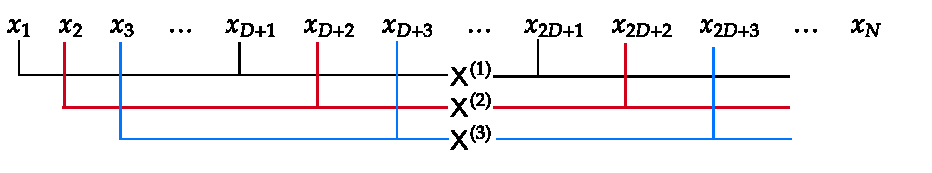
\includegraphics[width=\textwidth]{dstack_diagram.pdf}
  \caption{Визуализация Dstack преобразования одномерного ряда в многомерный.}
  \label{fig:dstack-diagram}
\end{figure}

\begin{theorem}
  Рассмотрим алгоритмы ESPRIT и HO-ESPRIT для многомерных рядов с
  выбором длины окна $L$,
  применённые к результату преобразования Dstack одномерного ряда
  $\tX$ с параметром $D$.
  Тогда между частотами $\omega$ в исходном ряде и оценками
  $\widetilde{\omega}$ частот преобразованного ряда существует
  взаимно однозначное соответствие тогда и только тогда, когда
  \begin{enumerate}
    \item  $\omega_i \ne \omega_j\ \forall i\ne j$,
    \item  $\min(L, N_D - L + 1) > \operatorname{rank}(\tX)$
    \item
      \begin{equation*}
        \max_{\omega \in \Omega}\omega \leqslant \frac{1}{2D},
      \end{equation*}
  \end{enumerate}
  причём это соответствие задаётся выражением
  \begin{equation*}
    \omega = \frac{|\widetilde{\omega}|}{D}.
  \end{equation*}
\end{theorem}
\begin{proof}
  Достаточно доказать, что указанные условия равносильны тому, что в
  пространстве подрядов $\tX_D^{(d)}$ длины $L$
  существует базис из векторов вида
  \begin{gather*}
    \left\{\left(e^{-\alpha n}\cos(2\pi n
      D\omega)\right)_{n=1}^{L},\, \omega \in
    \Omega,\, \alpha \in \bbR \right\},\\
    \left\{\left(e^{-\alpha n }\sin(2\pi n
      D\omega)\right)_{n=1}^{L},\, \omega \in
    \Omega \setminus\{1/2\},\, \alpha \in \bbR\right\}.
  \end{gather*}

  Элементы ряда $\tX_D^{(d)}$ имеют вид
  \begin{align*}
    x_n^{(d)} &= \sum_{i=1}^{M} a_i e^{-\alpha_i ((n - 1)D + d)}
    \cos(2 \pi ((n - 1)D + d) \omega_i + \varphi_i) \\
    &=\sum_{i=1}^{M} a_i e^{-\alpha_i(d - D)} e^{-\alpha_i nD }
    \cos(2 \pi nD \omega_i + \omega_i (d - D) + \varphi_i).
  \end{align*}
  Тогда существование искомого базиса равносильно тому, что длина $L$
  каждого подряда больше размерности этого базиса, то есть больше
  $\operatorname{rank}(\tX)$, и количество $K = N_D - L + 1$ таких подрядов тоже
  больше $\operatorname{rank}(\tX)$.
\end{proof}
\begin{corollary}
  Из доказательства следует, что всегда существует взаимно
  однозначное соответствие между степенями затухания $\alpha$ исходного ряда и
  оценками степеней затухания $\widetilde{\alpha}$ методами ESPRIT и
  HO-ESPRIT после применения преобразования Dstack,
  и это соответствие выражается как $\alpha = \widetilde{\alpha} / D$.
\end{corollary}
\begin{corollary}
  Так как в пространствах подрядов каждого ряда $\tX_D^{(d)}$
  существует нужный базис, то в методе HO-ESPRIT выбор параметра $R_3
  < \operatorname{rank}_3(\calX_D)$, где $\calX$ "--- траекторный
  тензор $\tX_D$, не даёт смещения в оценке параметров.
  Это отличительная особенность задачи оценки параметров, в
  задаче выделения сигнала выбор $R_3 < \operatorname{rank}_3(\calX)$ даёт
  смещение всегда.
\end{corollary}
\end{document}